\documentclass[journal]{IEEEtran}
% Report 2 (Labs 5-8), CS605 Artificial Intelligence, IIIT Vadodara, Autumn 2026-27.
% Written for the IEEE Transactions on Systems, Man, and Cybernetics: Systems LaTeX
% template (IEEEtran, journal mode). To use the course template, paste the body of
% this file into it and keep refs.bib and figures/ alongside.
\usepackage{amsmath,amssymb,amsfonts}
\usepackage{graphicx}
\usepackage{booktabs}
\usepackage{multirow}
\usepackage{algorithm}
\usepackage{algpseudocode}
\usepackage{cite}
\usepackage{url}
\usepackage[hidelinks]{hyperref}
\graphicspath{{figures/}}
\newcommand{\st}[1]{\texttt{#1}}

\begin{document}

\title{Reasoning and Deciding Under Uncertainty: Hidden Markov Models, Hopfield Networks,
Bandits and Markov Decision Processes}

\author{[Student Name 1, Roll No.],~[Student Name 2, Roll No.],~[Student Name 3, Roll No.],~[Student Name 4, Roll No.]%
\thanks{CS605 Artificial Intelligence, Lab Report 2 (Labs 5--8), Group [XX], IIIT Vadodara, Autumn 2026--27. Instructor: Pratik Shah. Code: [group Git repository URL].}}

\markboth{CS605 Artificial Intelligence --- Lab Report 2}{Group [XX]}

\maketitle

\begin{abstract}
This report is a tutorial on the second half of the CS605 laboratory. We fit Gaussian hidden
Markov models to twenty years of daily S\&P~500 and NASDAQ returns, recover calm and turbulent
market regimes whose dates match the 2000--02 and 2008--09 crises, and use the transition
matrix to forecast the regime. We build a $10\times10$ Hopfield associative memory, measure its
storage capacity (about $0.11N$--$0.14N$ patterns) and error-correcting radius, design an energy
function that solves the eight-rook problem in every one of 200 trials, and show why the
Hopfield--Tank network for a 10-city travelling salesman problem returns valid tours only
20--42\,\% of the time. We reimplement MENACE, the matchbox tic-tac-toe learner (which needs
exactly Michie's 304 boxes), and study exploration in stationary and non-stationary bandits,
where a constant step size raises the optimal-action rate from 47\,\% to 77--80\,\%. Finally we
solve the $4\times3$ grid world by value iteration for five reward settings and the Gbike
bicycle-rental MDP, in its original and modified forms, by policy iteration.
\end{abstract}

\begin{IEEEkeywords}
Hidden Markov model, Baum--Welch, Viterbi, market regimes, Hopfield network, associative
memory, combinatorial optimisation, MENACE, multi-armed bandit, $\epsilon$-greedy, Markov
decision process, value iteration, policy iteration.
\end{IEEEkeywords}

%=====================================================================================
\section{Introduction}
%=====================================================================================
\IEEEPARstart{T}{he} search problems of the first half of the course assumed that the agent
knows the state and the effect of its actions. The four labs in this report drop those
assumptions one at a time. In Lab~5 the state is \emph{hidden} and must be inferred from noisy
observations. In Lab~6 computation is done by a \emph{dynamical system} whose energy we design.
In Lab~7 the effects of actions are \emph{unknown} and must be learned from rewards. In Lab~8 the
effects are known but \emph{stochastic}, and the agent must plan a policy rather than a path. All
code is in Python, seeded for reproducibility, and every number below comes from the
accompanying scripts.

%=====================================================================================
\section{Lab 5: Market Regimes With a Gaussian HMM}
%=====================================================================================
\subsection{Model}
A hidden Markov model \cite{rabiner1989} has a hidden state $z_t\in\{1,\dots,K\}$ that evolves
as a Markov chain and an observation $x_t$ that depends only on the current state:
\begin{align}
\Pr(z_1=i) &= \pi_i, \qquad \Pr(z_{t+1}=j\mid z_t=i) = A_{ij},\\
x_t \mid z_t = k &\sim \mathcal{N}\bigl(\mu_k,\sigma_k^2\bigr).
\end{align}
For financial returns the hidden state is the market \emph{regime}, an idea that goes back to
Hamilton's regime-switching model \cite{hamilton1989}: in a calm regime returns have a small
spread, in a turbulent one a large spread, and regimes persist, so $A_{kk}$ is close to 1.

The parameters $\theta = (\pi, A, \mu, \sigma)$ are fitted by Baum--Welch, the EM algorithm
for HMMs. The E-step uses the forward--backward recursions to compute
$\gamma_t(k) = \Pr(z_t=k\mid x_{1:T})$ and
$\xi_t(i,j)=\Pr(z_t=i, z_{t+1}=j\mid x_{1:T})$; the M-step re-estimates
\begin{gather}
\hat A_{ij} = \frac{\sum_t \xi_t(i,j)}{\sum_t \gamma_t(i)},\qquad
\hat\mu_k = \frac{\sum_t \gamma_t(k)\,x_t}{\sum_t\gamma_t(k)},\\
\hat\sigma_k^2 = \frac{\sum_t \gamma_t(k)(x_t-\hat\mu_k)^2}{\sum_t\gamma_t(k)} .
\end{gather}
EM only finds a local maximum of the likelihood, so we ran it from 10 random starts and kept
the best. The most likely state sequence is then found by the Viterbi algorithm. We used
\st{hmmlearn} \cite{hmmlearn} and sorted the states by variance so that state 0 is always the
calmest.

\subsection{Data and preprocessing}
The script first requests daily prices from the Yahoo Finance API. Our environment could not
reach Yahoo, so it fell back to the Yahoo-sourced daily data bundled with the \st{arch} package
\cite{arch}: S\&P~500 (\st{\^{}GSPC}) and NASDAQ Composite (\st{\^{}IXIC}) adjusted closes from
4 January 1999 to 31 December 2018. That is 5\,030 daily returns each, covering the dot-com
crash, the 2008 crisis and the 2011 and 2015--16 sell-offs. Running the script with internet
access refits the same models on data up to the present. Preprocessing removes duplicate dates,
forward-fills missing prices (none were found), and computes daily log returns in percent,
\begin{equation}
x_t = 100\,\ln\frac{P_t}{P_{t-1}} .
\end{equation}
Returns larger than 30\,\% in magnitude would be treated as data errors; none occurred. Log
returns are used because they add over time and are closer to Gaussian than prices, which are
non-stationary.

\subsection{Choosing the number of states}
More states always increase the likelihood, so we penalise model size with the Akaike and
Bayesian information criteria. With $p = (K-1) + K(K-1) + 2K$ free parameters and $T$
observations,
\begin{equation}
\mathrm{AIC} = -2\ln\hat L + 2p, \qquad \mathrm{BIC} = -2\ln\hat L + p\ln T \;\;\text{\cite{schwarz1978}}.
\end{equation}
Table~\ref{tab:hmmsel} shows that BIC picks $K=3$ for the S\&P~500 and $K=4$ for the NASDAQ.
The fourth S\&P state is a symptom of over-fitting: it has a standard deviation of 0.25\,\%,
an expected duration of 1.3 days and switches 230 times, so it describes short quiet spells
within the calm regime rather than a regime of its own.

\begin{table}[t]
\centering
\caption{Model selection (lower AIC/BIC is better)}\label{tab:hmmsel}
\begin{tabular}{@{}llrrr@{}}
\toprule
Index & $K$ & $\ln\hat L$ & AIC & BIC \\
\midrule
\multirow{3}{*}{S\&P 500} & 2 & $-7131.7$ & 14\,277.3 & 14\,323.0 \\
 & 3 & $-6900.7$ & 13\,829.5 & \textbf{13\,920.8} \\
 & 4 & $-6865.8$ & \textbf{13\,777.6} & 13\,927.6 \\
\midrule
\multirow{3}{*}{NASDAQ} & 2 & $-8451.1$ & 16\,916.2 & 16\,961.9 \\
 & 3 & $-8267.1$ & 16\,562.1 & 16\,653.5 \\
 & 4 & $-8204.7$ & \textbf{16\,455.4} & \textbf{16\,605.4} \\
\bottomrule
\end{tabular}
\end{table}

\subsection{The regimes}
Table~\ref{tab:hmmpar} lists the fitted parameters for the S\&P~500, annualised as
$252\mu_k$ and $\sqrt{252}\,\sigma_k$. With $K=2$ the model splits the market into a
\emph{low-volatility bull} state (annualised volatility 10.9\,\%, drift $+17.4\,\%$ per year,
66\,\% of days) and a \emph{high-volatility bear} state (28.7\,\%, $-22.2\,\%$, 34\,\% of days).
Volatility, not the mean, separates the states: the two means differ by only 0.16 percentage
points a day, well inside one standard deviation, whereas the variances differ by a factor of
seven. This matches the well-known ``volatility clustering'' of returns. Fig.~\ref{fig:spx2}
shows the decoded states. The longest bear spells are 5 June 2008--23 July 2009 (286 days) and
11 April 2002--28 April 2003 (264 days), followed by the start of 1999 and the run-up to the
2008 crisis (Oct.~2007--Apr.~2008). The low-volatility state covers the long rallies of
2003--07 and 2012--17.

\begin{table}[t]
\centering
\caption{Gaussian HMM parameters for S\&P 500 daily log returns}\label{tab:hmmpar}
\setlength{\tabcolsep}{2.6pt}
\begin{tabular}{@{}llrrrrrr@{}}
\toprule
$K$ & state & $\mu_k$ (\%) & $\sigma_k$ (\%) & ann.\ mean & ann.\ vol & $1/(1-A_{kk})$ & share \\
\midrule
2 & 0 bull & 0.069 & 0.685 & $+17.4\,\%$ & 10.9\,\% & 83 d & 66\,\% \\
  & 1 bear & $-0.088$ & 1.806 & $-22.2\,\%$ & 28.7\,\% & 44 d & 34\,\% \\
\midrule
3 & 0 calm & 0.091 & 0.548 & $+23.1\,\%$ & 8.7\,\% & 48 d & 45\,\% \\
  & 1 normal & $-0.024$ & 1.167 & $-6.1\,\%$ & 18.5\,\% & 37 d & 46\,\% \\
  & 2 crisis & $-0.160$ & 2.665 & $-40.3\,\%$ & 42.3\,\% & 32 d & 9\,\% \\
\bottomrule
\end{tabular}
\end{table}

\begin{figure}[t]
\centering
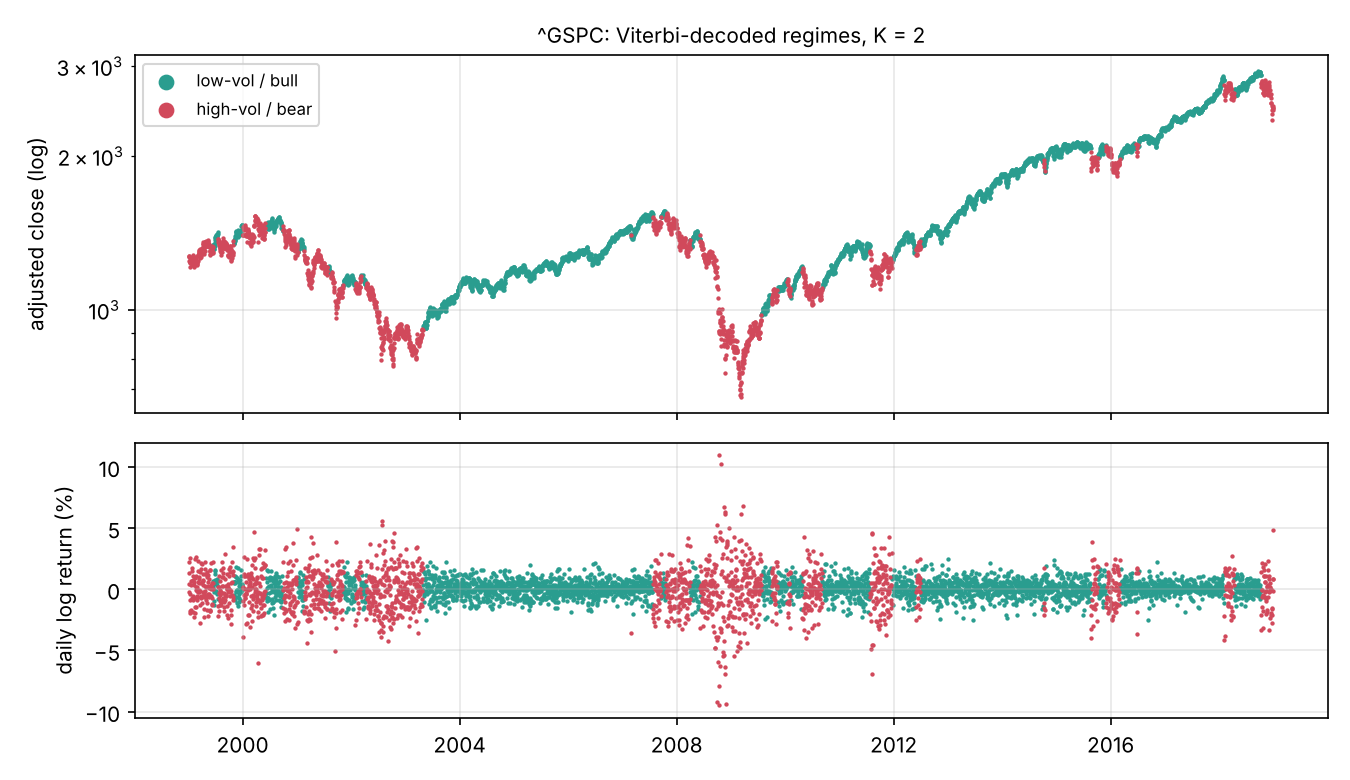
\includegraphics[width=\columnwidth]{spx_regimes_k2.png}
\caption{S\&P 500 (1999--2018) coloured by the Viterbi state of the two-state HMM. Top: adjusted
close (log scale); bottom: daily log returns.}
\label{fig:spx2}
\end{figure}

With $K=3$ the bear state splits into a ``normal'' state (18.5\,\% volatility) and a
\emph{crisis} state (42.3\,\% volatility, 9\,\% of days) whose longest spells are
4 September 2008--18 May 2009, August--November 2011 (the U.S.\ downgrade and euro-zone crisis)
and July--October 2002 (Fig.~\ref{fig:spx3}). The NASDAQ gives the same picture with higher
volatility in every state (14.3\,\% and 37.9\,\% for $K=2$), and its two-state model assigns the
entire dot-com bust, 5 January 1999--2 April 2003 (1\,066 days), to the high-volatility state.
Technology stocks were turbulent for far longer than the broad market.

\begin{figure}[t]
\centering
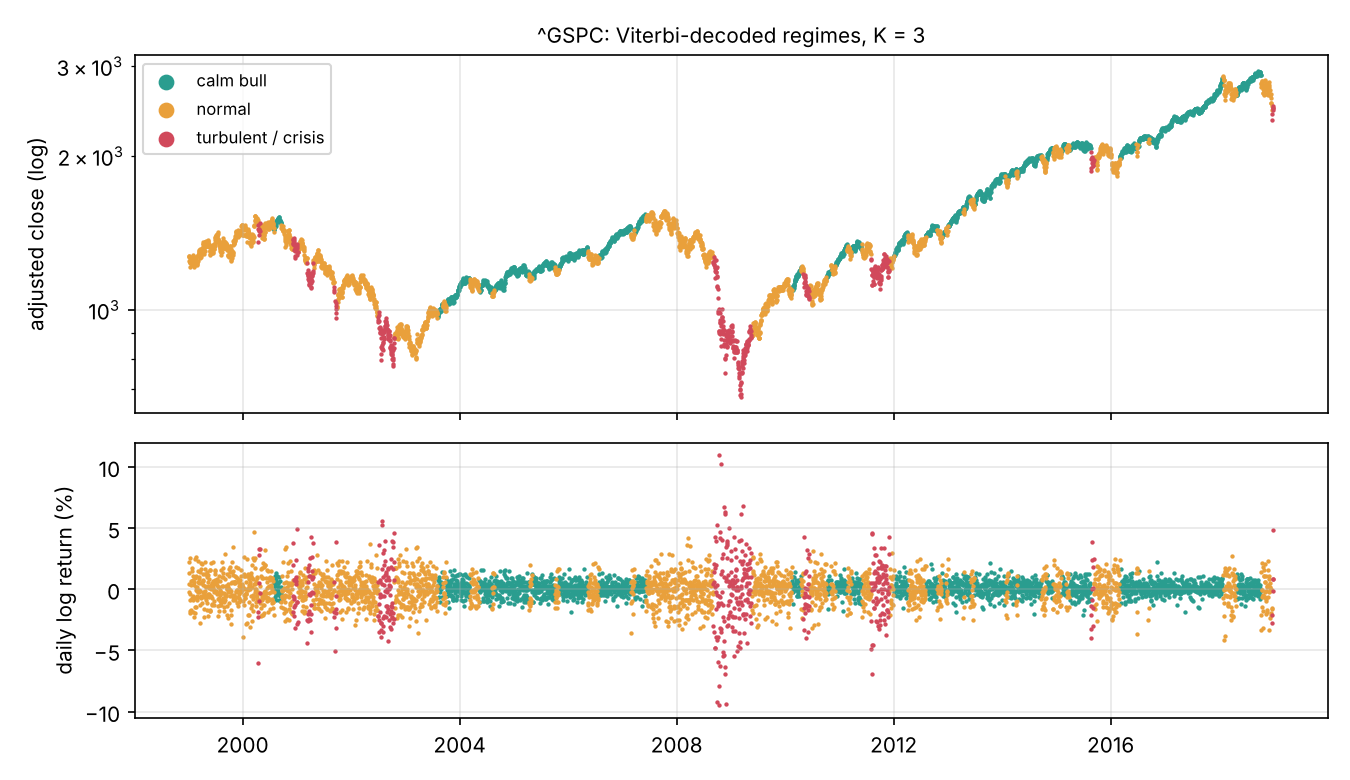
\includegraphics[width=\columnwidth]{spx_regimes_k3.png}
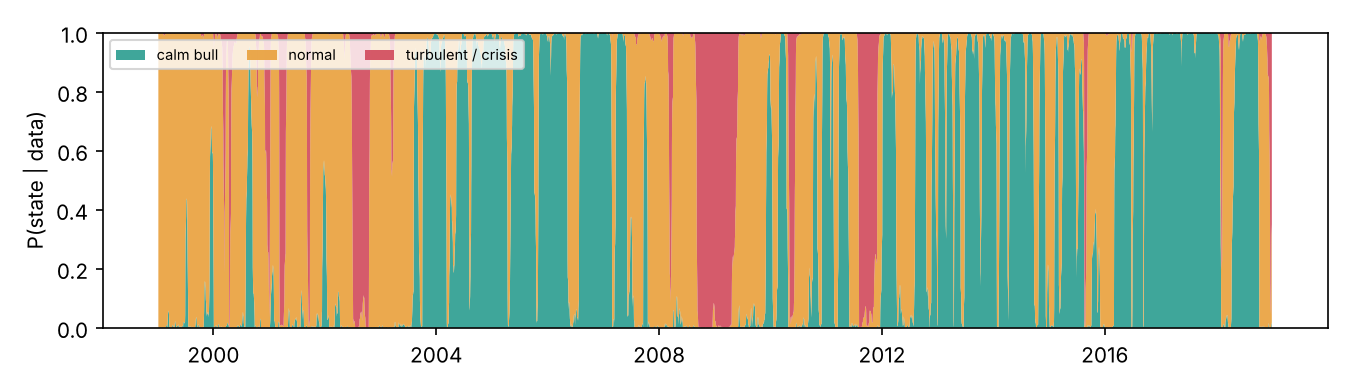
\includegraphics[width=\columnwidth]{spx_posterior_k3.png}
\caption{Three-state model. Top: Viterbi states. Bottom: posterior state probabilities
$\gamma_t(k)$ from forward--backward, which show how confident the model is about each day.}
\label{fig:spx3}
\end{figure}

\subsection{Transition matrix and expected durations}
For the two-state S\&P model,
\begin{equation}
A = \begin{bmatrix} 0.9880 & 0.0120 \\ 0.0226 & 0.9774 \end{bmatrix}.
\end{equation}
A regime lasts a geometrically distributed number of days with mean $1/(1-A_{kk})$: about 83
trading days for the bull state and 44 for the bear state. The stationary distribution, the
solution of $\boldsymbol{\pi}^\top A = \boldsymbol{\pi}^\top$, is $(0.652, 0.348)$, close to the
observed shares. In the three-state model the crisis state is reached almost only from the
normal state ($A_{0,2}=0.0003$ against $A_{1,2}=0.0066$) and is left only towards it
($A_{2,0}\approx0$), so the market passes through ``normal'' on its way into and out of a crisis.

\subsection{Forecasting the regime}
The filtered probability of the last day, $\mathbf{p}_T$, propagates through the chain as
\begin{equation}
\mathbf{p}_{T+h}^\top = \mathbf{p}_T^\top A^{h}.
\end{equation}
On 31 December 2018, after the sharp fall of late 2018, the two-state model put 78\,\%
probability on the bear state. The forecast is 77\,\% one day ahead, 71\,\% one week ahead,
56\,\% one month (21 trading days) ahead and 40\,\% one quarter ahead, decaying towards the
stationary 35\,\%. The three-state model gives 65\,\% crisis probability, falling to 38\,\% in a
month. The data end there, so this forecast cannot be checked within the sample; refitting on data up
to the present would allow it.
Such forecasts are most useful for \emph{risk} decisions, for example scaling exposure by the
predicted volatility $\sum_k p_{T+h}(k)\,\sigma_k$, rather than for predicting the direction of
the market, because the state means are small and noisy.

\subsection{Evaluation}
The HMM explains returns much better than a single Gaussian: the mixture of a narrow and a wide
component reproduces the sharp peak and the fat tails of the return histogram (Fig.~\ref{fig:hist}),
and the log-likelihood rises from $-8\,069.9$ for a single Gaussian ($K=1$) to $-7\,131.7$ for
$K=2$, a gain of 938 for only four extra parameters. The model has clear limitations,
however. Volatility in reality changes gradually (as in GARCH models) rather than jumping between
a few levels. The Gaussian emissions still underestimate the extreme days of October 2008. The
regimes are identified after the fact, while the filtered probability reacts with a lag of a few
days. And the parameters are assumed constant over twenty years.

\begin{figure}[t]
\centering
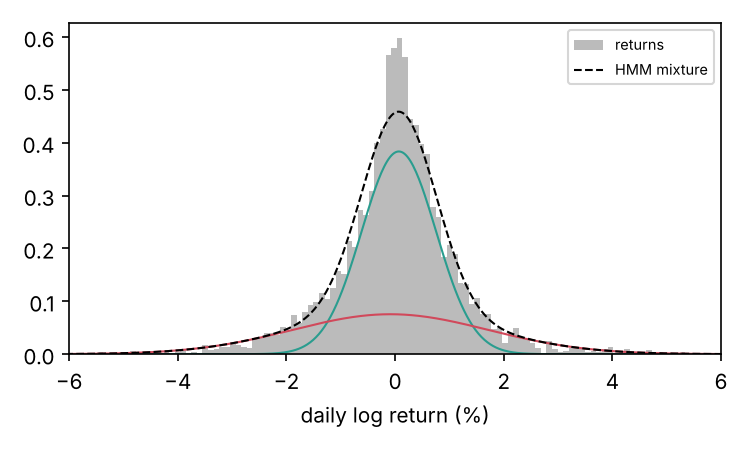
\includegraphics[width=0.75\columnwidth]{spx_hist_k2.png}
\caption{Histogram of S\&P 500 daily returns with the two Gaussian components of the HMM,
weighted by state occupancy, and their mixture.}
\label{fig:hist}
\end{figure}

%=====================================================================================
\section{Lab 6: Hopfield Networks}
%=====================================================================================
\subsection{The network}
A Hopfield network \cite{hopfield1982,mackay2003} has $N$ bipolar units $s_i\in\{-1,+1\}$ and
symmetric weights $w_{ij}=w_{ji}$ with $w_{ii}=0$. Units are updated one at a time
(asynchronously):
\begin{equation}
s_i \leftarrow \operatorname{sgn}\Bigl(\sum_j w_{ij}s_j\Bigr).
\end{equation}
Each such update can only lower, or keep, the energy
\begin{equation}
E(\mathbf{s}) = -\tfrac12 \sum_{i,j} w_{ij}s_is_j ,
\end{equation}
so the network always settles in a local minimum. To store patterns
$\boldsymbol{\xi}^{1},\dots,\boldsymbol{\xi}^{P}$ we use the Hebbian rule
\begin{equation}
w_{ij} = \frac1N\sum_{\mu=1}^{P}\xi_i^\mu\xi_j^\mu \quad (i\ne j),
\end{equation}
which makes each stored pattern a low-energy state. Recall starts the network at a corrupted
probe and lets it fall into the nearest minimum.

\subsection{A $10\times10$ associative memory}
We stored five $10\times10$ letter glyphs (A, T, X, O, L; $N=100$, so 4\,950 independent weights).
Flipping 20 of the 100 pixels and running asynchronous updates restored every letter exactly
(Fig.~\ref{fig:letters}); the energy fell from about $-17$ to $-25$ for the probes to $-51$ to
$-64$ for the recalled letters. Real glyphs are correlated (the overlap
$\frac1N\boldsymbol{\xi}^\mu\cdot\boldsymbol{\xi}^\nu$ reaches $-0.44$ for X and O), which
reduces capacity compared with random patterns.

\begin{figure}[t]
\centering
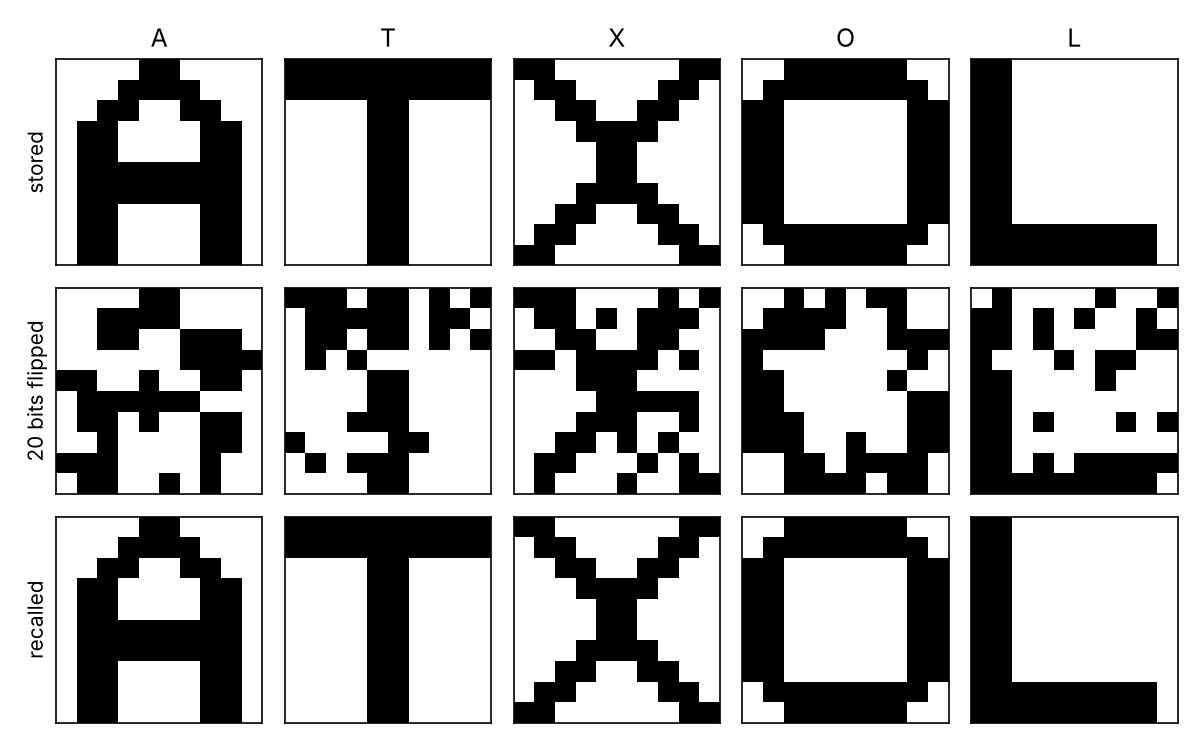
\includegraphics[width=0.9\columnwidth]{hopfield_letters.png}
\caption{Associative recall: stored glyphs, probes with 20 \% of pixels flipped, and the
recalled states.}
\label{fig:letters}
\end{figure}

\subsection{Capacity}
For random patterns, the input to unit $i$ when the network is in pattern $\mu$ is the signal
$\xi_i^\mu$ plus crosstalk from the other $P-1$ patterns, which is approximately Gaussian with
variance $(P-1)/N$. A bit is stable when the crosstalk does not overturn the signal, so the
bit-error probability is approximately
\begin{equation}
P_{\mathrm{err}} \approx \Phi\Bigl(-\sqrt{N/P}\Bigr).
\end{equation}
Requiring all bits of all patterns to be stable gives $P_{\max}\approx N/(2\ln N)\approx10.9$
for $N=100$ \cite{mceliece1987}; allowing a small fraction of bit errors raises it to the
statistical-mechanics limit $0.138N\approx14$ \cite{amit1985}. Our experiment
(Fig.~\ref{fig:capacity}, 20 trials per $P$) agrees: every pattern is a fixed point up to
$P=8$, 89\,\% at $P=12$, 78\,\% at $P=14$ and 38\,\% at $P=20$, while more than 98.9\,\% of the
individual bits remain stable even at $P=20$. Recall from a clean probe succeeds (to within one
bit) 95\,\% of the time up to $P=13$ and breaks down beyond $P\approx 0.14N$. So a $10\times10$
network stores about 10--14 distinct random patterns reliably.

\begin{figure}[t]
\centering
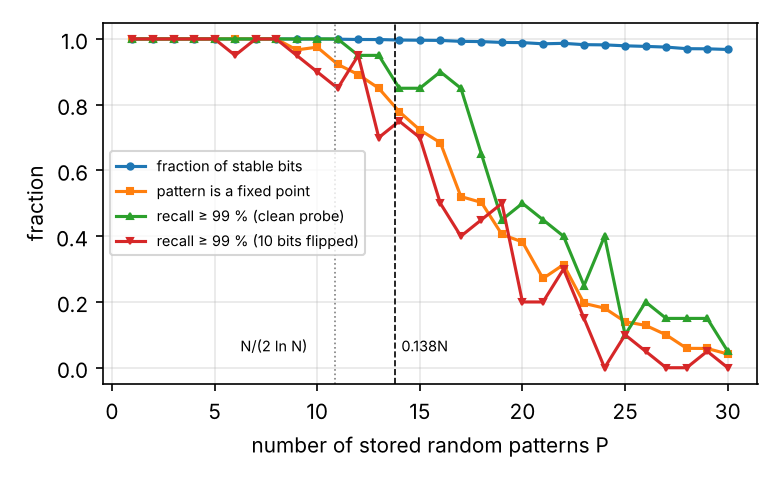
\includegraphics[width=0.95\columnwidth]{hopfield_capacity.png}
\caption{Capacity of a 100-unit Hopfield network for random patterns.}
\label{fig:capacity}
\end{figure}

\subsection{Error-correcting capability}
Fig.~\ref{fig:errcorr} shows the probability of \emph{exact} recall when $k$ bits of a stored
pattern are flipped (60 trials per point). With a single stored pattern the network corrects up
to 48 flipped bits, because any probe with fewer than $N/2$ errors still has positive overlap with
the pattern; beyond 50 it falls into the inverted pattern $-\boldsymbol{\xi}$, which is also a
minimum. As more patterns compete, the basins shrink: the largest $k$ that is corrected at least
90\,\% of the time is 36 bits for $P=3$, 32 for $P=5$, 26 for $P=8$ and 20 for $P=10$, and at
$P=12$ even a clean probe is not always stable. A useful rule of thumb from these results is
that a lightly loaded network ($P\le0.05N$) corrects about a third of the bits.

\begin{figure}[t]
\centering
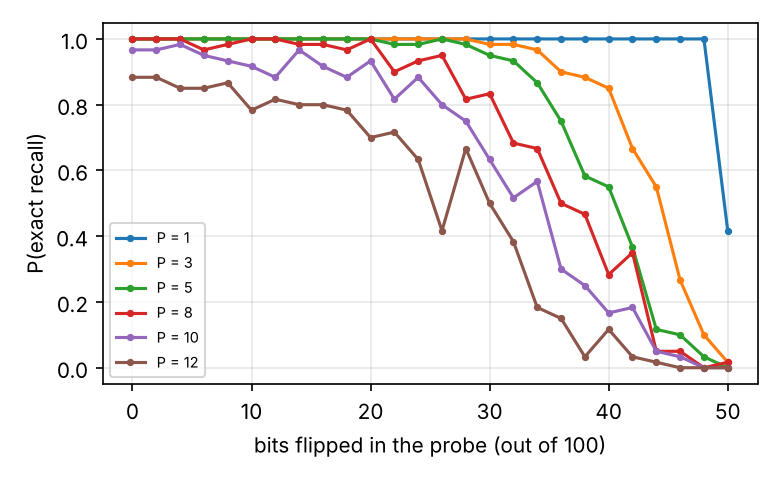
\includegraphics[width=0.95\columnwidth]{hopfield_error_correction.png}
\caption{Exact recall probability against the number of flipped bits, for several loads $P$.}
\label{fig:errcorr}
\end{figure}

\subsection{The eight-rook problem}
To optimise with a Hopfield network we write the constraints as an energy and read off the
weights. Let $v_{ij}\in\{0,1\}$ mean ``a rook on square $(i,j)$''. Eight non-attacking rooks need
exactly one rook in every row and every column:
\begin{equation}
E = \frac{A}{2}\sum_{i}\Bigl(\sum_j v_{ij}-1\Bigr)^2 + \frac{B}{2}\sum_j\Bigl(\sum_i v_{ij}-1\Bigr)^2 .
\end{equation}
Expanding the squares with $v^2=v$ gives, up to a constant,
\begin{equation}
E = \frac A2\sum_i\sum_{j\ne l}v_{ij}v_{il} + \frac B2\sum_j\sum_{i\ne k}v_{ij}v_{kj}
    - \frac{A+B}{2}\sum_{i,j}v_{ij}.
\end{equation}
Matching this with the Hopfield energy $E=-\frac12\sum w\,v\,v - \sum I\,v$ gives the weights
and biases
\begin{gather}
w_{(ij),(kl)} = -A\,\delta_{ik}(1-\delta_{jl}) - B\,\delta_{jl}(1-\delta_{ik}),\\
I_{ij} = \frac{A+B}{2}.
\end{gather}
Each unit inhibits the 14 others in its row and column, so the network has 448 non-zero
symmetric weights out of $64\times63/2$. We chose $A=B=2$ for the following reason. A unit turns
on when its net input $2 - 2r - 2c$ is positive, where $r$ and $c$ are the numbers of rooks
already in its row and column. So it turns on only if both are empty, and turns off if either is
occupied. Hence every stable state has at most one rook per row and column and no empty row
paired with an empty column: it is a solution. Equal row and column weights are natural because
the two constraints are symmetric, and the bias equal to half the total inhibition places the
threshold between ``no conflict'' and ``one conflict''. From 200 random initial states the
network reached a valid placement every time, in three sweeps on average, always at the energy
minimum $E=-16$, and the 200 runs produced 200 different solutions out of the $8!=40\,320$
possible.

\subsection{TSP with the Hopfield--Tank network}
For $n$ cities, Hopfield and Tank \cite{hopfieldtank1985} use $n^2$ units: $V_{x,i}\in[0,1]$
means ``city $x$ is visited at position $i$''. The energy is
\begin{equation}
\begin{split}
E = {}&\frac A2\sum_x\sum_i\sum_{j\ne i}V_{xi}V_{xj} + \frac B2\sum_i\sum_x\sum_{y\ne x}V_{xi}V_{yi}\\
  &+ \frac C2\Bigl(\sum_{x,i}V_{xi} - n'\Bigr)^2 \\
  &+ \frac D2\sum_x\sum_{y\ne x}\sum_i d_{xy}V_{xi}\bigl(V_{y,i+1}+V_{y,i-1}\bigr),
\end{split}
\end{equation}
where the $A$ term forbids a city in two positions, $B$ two cities in one position, $C$ forces
$n'$ active units, and $D$ adds the tour length. The corresponding weights are
\begin{multline}
T_{xi,yj} = -A\delta_{xy}(1-\delta_{ij}) - B\delta_{ij}(1-\delta_{xy}) - C \\
- D\,d_{xy}\bigl(\delta_{j,i+1}+\delta_{j,i-1}\bigr),
\end{multline}
with bias $I_{xi}=Cn'$. For 10 cities the network therefore needs $n^2=100$ neurons and a
$100\times100=10\,000$-entry weight matrix, of which 9\,900 off-diagonal entries are non-zero
($100\cdot99/2=4\,950$ independent symmetric weights) plus 100 biases; in general $O(n^4)$ weights.
We integrated $\dot u = -u + T V + I$ with $V=\frac12(1+\tanh(u/u_0))$, using the original
parameters $A=B=500$, $C=200$, $D=500$, $n'=15$ and $u_0=0.02$, on 10 random cities in the unit
square whose optimum (by brute force over $9!/2$ tours) is 2.962.

With these parameters only 10 of 50 runs gave a valid permutation matrix; the valid tours were
on average 15.8\,\% longer than optimal and the best was 3.1\,\% above it
(Fig.~\ref{fig:hoptsp}). Varying $D$ exposes the trade-off that Wilson and Pawley reported
\cite{wilson1988} (Table~\ref{tab:hoptsp}): a weak distance term gives more valid but worse
tours, a strong one gives better tours but rarely a valid one, and at $D=700$ no run was valid.
The penalty method makes the constraints and the objective compete inside one energy, so
the minima of $E$ need not be valid tours. That is why, unlike the eight-rook network, whose
energy contains only constraints, the TSP network is unreliable. Simulated annealing with 2-opt moves, which found the exact optimum
of a 20-city tour in Report~1, is the better tool for this problem.

\begin{table}[t]
\centering
\caption{Hopfield--Tank TSP, 10 cities, 50 runs per setting}\label{tab:hoptsp}
\begin{tabular}{@{}rccc@{}}
\toprule
$D$ & valid tours & mean length / optimum & best / optimum \\
\midrule
200 & 36\,\% & 1.292 & 1.100 \\
300 & 42\,\% & 1.258 & 1.031 \\
500 & 20\,\% & 1.158 & 1.031 \\
700 & 0\,\% & -- & -- \\
\bottomrule
\end{tabular}
\end{table}

\begin{figure}[t]
\centering
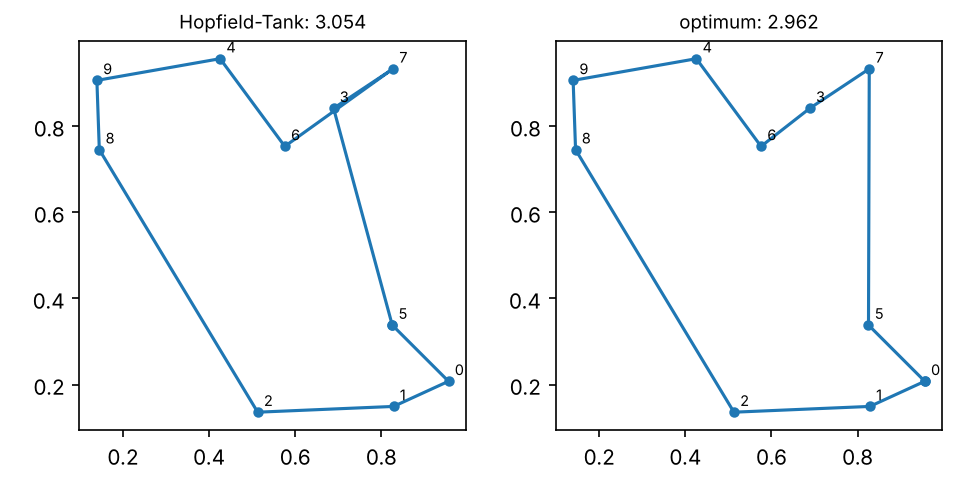
\includegraphics[width=0.9\columnwidth]{hopfield_tsp.png}
\caption{Best Hopfield--Tank tour ($D=500$) and the optimal tour.}
\label{fig:hoptsp}
\end{figure}

%=====================================================================================
\section{Lab 7: Learning From Reward}
%=====================================================================================
\subsection{MENACE}
Michie's MENACE \cite{michie1963} learns noughts and crosses with matchboxes and coloured beads.
There is one box for every position MENACE (playing X, moving first) can face, and one bead colour
for each legal move. To move, MENACE draws a bead at random; after the game every bead drawn is
reinforced. In modern terms the bead counts define a stochastic policy
$\pi(a\mid s)\propto n_{s,a}$, and reinforcement is a crude Monte-Carlo policy update.

We wrote our own Python implementation after reading the reference. The parts that matter most
are the following.
\begin{itemize}
\item \emph{Symmetry reduction} (\st{canonical}). Each board is mapped to the lexicographically
smallest of its eight rotations and reflections, and the chosen move is mapped back through the
same permutation. This is what makes the machine small enough to build out of matchboxes:
counting all non-terminal positions with X to move gives 338 canonical boxes, and dropping the 34
positions with a single empty square (where the move is forced) gives exactly Michie's 304. Moves
that are symmetric inside a position (e.g.\ the four corners of the empty board) share one bead
colour, so the first box holds only three: centre, corner and edge.
\item \emph{Initial beads} by stage of the game: 4, 3, 2, 1 beads per move for MENACE's first,
second, third and fourth moves, so that later, more decisive choices change faster.
\item \emph{Reinforcement} (\st{reinforce}): $+3$ beads for a win, $+1$ for a draw and $-1$ for a
loss, applied to every (box, bead) pair of the game. This solves the credit-assignment problem
in the simplest way, by giving every move the outcome of the whole game.
\item \emph{Empty boxes}: if a box runs out of beads MENACE resigns (a loss), and the box is
refilled so that the position is not permanently lost.
\end{itemize}
Against a random opponent MENACE's win rate rises from 68\,\% in the first 100 games to 86\,\% in
the last 500 of 3\,000 games (mean of five runs), and losses fall from 22\,\% to 6\,\%. Against a
perfect minimax opponent MENACE loses 34\,\% of its first 100 games; by the end losses have
vanished and 99.96\,\% of the last 500 games are draws (Fig.~\ref{fig:menace}). The trained machine
opens in the centre: after training against the perfect player the first box holds 2\,960 centre
beads and none for corners or edges, because those openings were punished.

\begin{figure}[t]
\centering
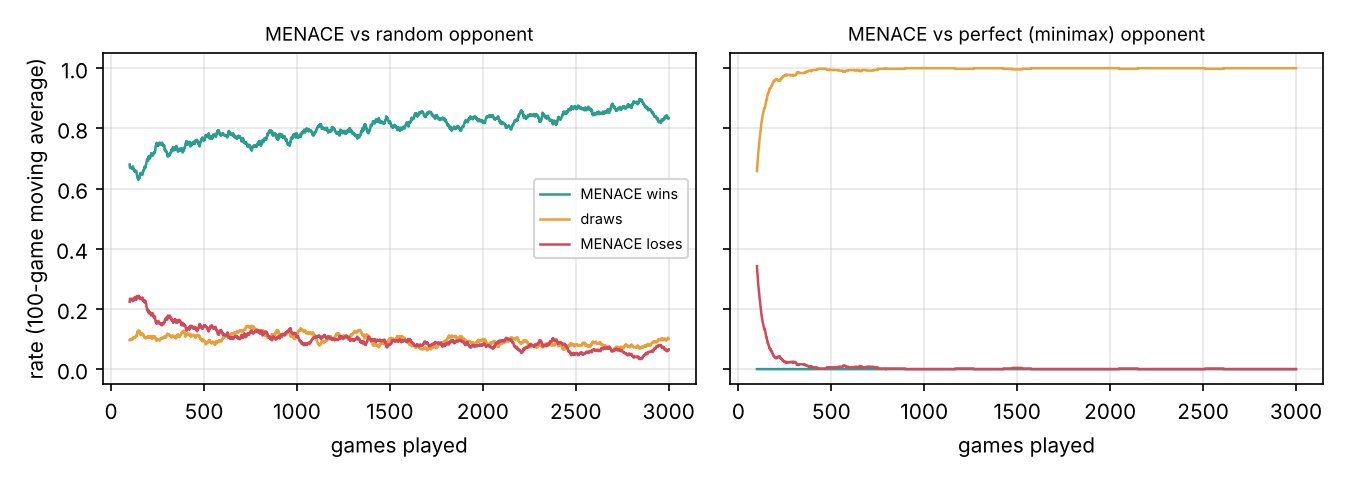
\includegraphics[width=\columnwidth]{menace_learning.png}
\caption{MENACE learning curves (100-game moving averages, mean of five runs).}
\label{fig:menace}
\end{figure}

\subsection{Binary bandits and $\epsilon$-greedy}
A bandit has $k$ actions with unknown reward distributions; the agent must balance
\emph{exploiting} the action that looks best with \emph{exploring} the others \cite{sutton2018}.
The $\epsilon$-greedy agent keeps an estimate $Q(a)$ for each action, takes the greedy action
$\arg\max_a Q(a)$ with probability $1-\epsilon$ and a uniformly random action otherwise, and
updates the estimate of the chosen action with the incremental sample average
\begin{equation}
Q_{n+1}(a) = Q_n(a) + \frac{1}{n}\bigl(R_n - Q_n(a)\bigr).
\end{equation}
\st{binaryBanditA} and \st{binaryBanditB} from the course repository \cite{cs307repo}, ported to
Python, return reward 1 with probabilities $(0.1, 0.2)$ and $(0.8, 0.9)$ for actions 1 and 2.
Both are hard in the same way: the two actions differ by only 0.1. We averaged 2\,000 runs of
1\,000 steps (Fig.~\ref{fig:binary}). With $\epsilon=0.1$ the agent picks action 2 in 94\,\% of
the last 200 steps on both bandits and earns 0.194 (A) and 0.894 (B) per step, against the best
possible 0.2 and 0.9. The purely greedy agent ($\epsilon=0$) locks onto whichever action happens
to pay first and chooses correctly only 67\,\% (A) and 52\,\% (B) of the time; on bandit B, where
both actions usually pay, it is barely better than chance. $\epsilon=0.2$ explores too much
(90\,\% optimal), and $\epsilon=0.01$ learns slowly (82--85\,\% after 1\,000 steps).

\begin{figure}[t]
\centering
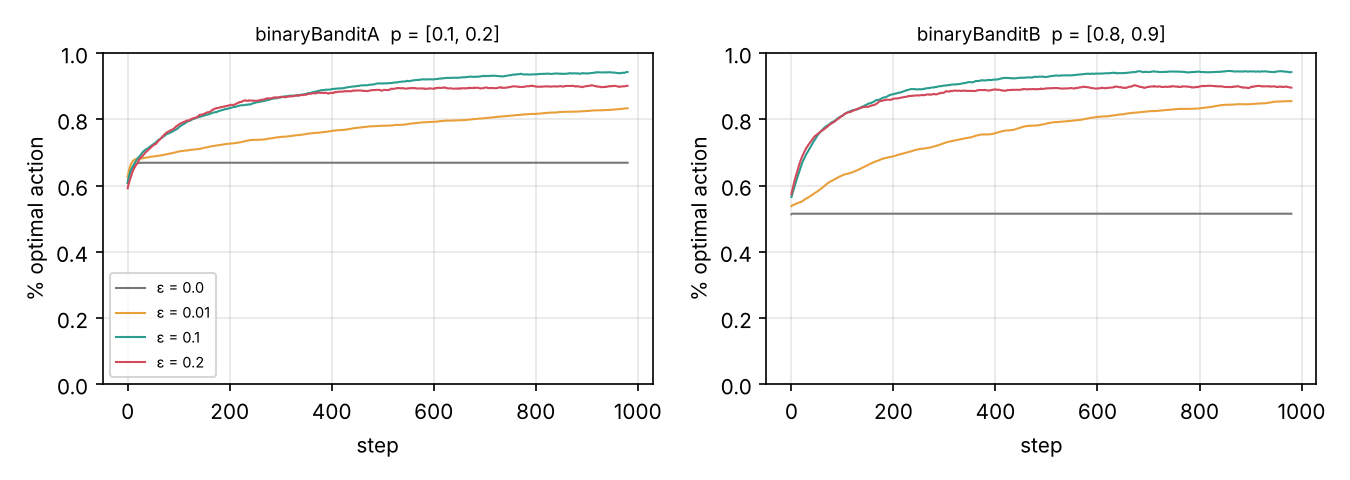
\includegraphics[width=\columnwidth]{binary_bandits.png}
\caption{Fraction of runs choosing the better action on binaryBanditA and binaryBanditB.}
\label{fig:binary}
\end{figure}

\subsection{A non-stationary 10-armed bandit}
\st{bandit\_nonstat} has ten arms whose mean rewards $q_*(a)$ all start at 0 and take independent
random walks, and returns a reward drawn around the current mean of the chosen arm:
\begin{gather}
q_*(a) \leftarrow q_*(a) + \eta_a,\qquad \eta_a\sim\mathcal{N}(0, 0.01^2),\\
R_t \sim \mathcal{N}\bigl(q_*(A_t), 1\bigr).
\end{gather}
After 10\,000 steps the means are spread over about 4 units, and in one sample run the identity of
the best arm changed 158 times (Fig.~\ref{fig:nonstat}, right). The sample average weights a
reward from step 10 as much as one from step 10\,000, so it stops tracking the moving targets.
The fix \cite{sutton2018} is a constant step size $\alpha$:
\begin{equation}
Q_{n+1} = Q_n + \alpha(R_n - Q_n) = (1-\alpha)^{n}Q_1 + \sum_{i=1}^{n}\alpha(1-\alpha)^{n-i}R_i ,
\end{equation}
an exponential recency-weighted average with an effective memory of about $1/\alpha$ steps. It
no longer converges, but in a changing world that is exactly what is wanted.

Over 1\,000 runs of 10\,000 steps, with the same environment sequence for every agent, the sample
average agent ($\epsilon=0.1$) chose the currently best arm in only 47\,\% of the last 1\,000
steps, earning 1.10 per step. With $\alpha=0.1$ the same agent latched onto the right arm 77\,\%
of the time and earned 1.35; $\alpha=0.05$ performed the same; and reducing exploration to
$\epsilon=0.05$ with $\alpha=0.1$ gave the best result, 80\,\% and 1.43
(Fig.~\ref{fig:nonstat}, left). So the modified agent does latch onto the correct actions and
keeps re-latching as they change; the step size, not the amount of exploration, is what matters
most here.

\begin{figure}[t]
\centering
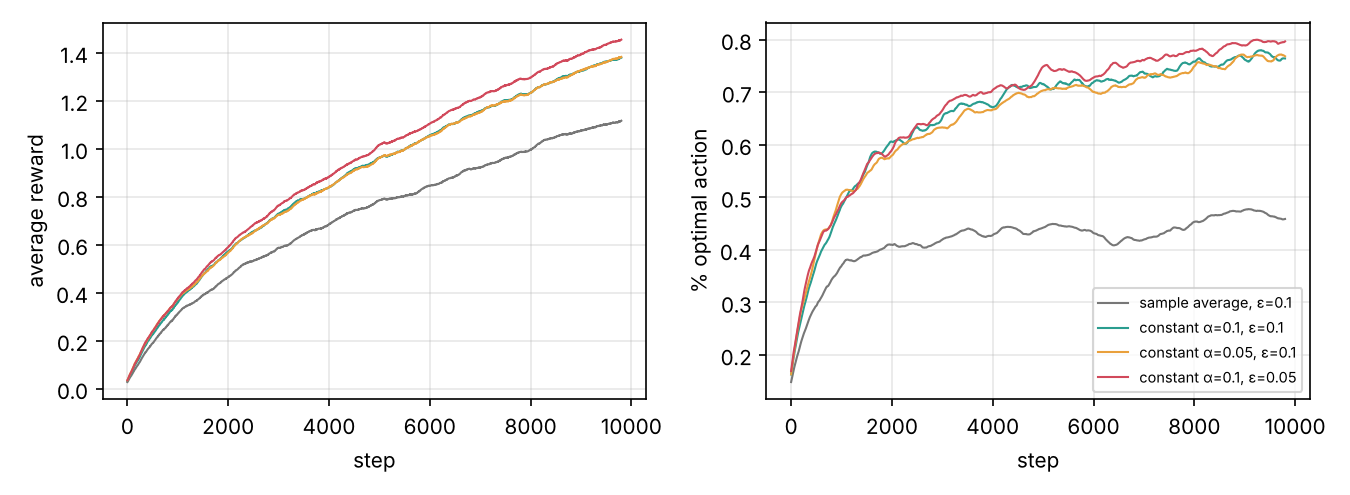
\includegraphics[width=\columnwidth]{nonstationary_bandit.png}
\caption{Non-stationary 10-armed bandit: average reward and optimal-action rate (200-step moving
averages over 1\,000 runs).}
\label{fig:nonstat}
\end{figure}

%=====================================================================================
\section{Lab 8: Markov Decision Processes}
%=====================================================================================
\subsection{Value iteration on the $4\times3$ world}
An MDP is a tuple $(S, A, P, R, \gamma)$. The utility of a state under the optimal policy satisfies
the Bellman equation \cite{bellman1957,aima4}
\begin{equation}
U(s) = R(s) + \gamma\max_{a}\sum_{s'}P(s'\mid s,a)\,U(s'),
\end{equation}
and value iteration applies it as an update to all states until the largest change falls below a
threshold. In the grid world of Fig.~\ref{fig:grid} each action goes in the intended direction with
probability 0.8 and at right angles with probability 0.1 each, a move into a wall leaves the agent
where it is, and the two exits pay $+1$ and $-1$. We use $\gamma=1$ when $R(s)<0$; then every
policy that avoids the exits has utility $-\infty$, so value iteration converges. When
$R(s)\ge0$ an agent can collect reward forever and the undiscounted utilities diverge, so for those
cases we use $\gamma=0.99$.

For $R(s)=-0.04$ value iteration converged in 28 sweeps to the utilities of the textbook,
$U(1,1)=0.705$, $U(3,3)=0.918$ and $U(4,1)=0.388$. The policy goes up and around through the top
row, and from $(3,1)$ and $(4,1)$ it goes left, the long way round, to avoid slipping into $-1$.
Changing the living reward changes the agent's attitude to risk:
\begin{itemize}
\item $R(s)=-2$: life is so costly that ending it at $-1$ is better. The agent heads straight for
the nearest exit; from $(3,2)$ it moves right into $-1$, and from $(4,1)$ it goes up into $-1$.
\item $R(s)=0.02$, $0.1$ and $1$: living is rewarding, so the agent avoids both exits for ever.
Every state has value $R/(1-\gamma)$ ($2$, $10$ and $100$); next to the exits it chooses actions
that cannot possibly reach them, such as left from $(3,3)$ and $(3,2)$ and down (into the wall)
from $(4,1)$. Elsewhere all actions are equally good.
\end{itemize}
Sweeping $R(s)$ from $-2$ to 0 in steps of 0.005 shows the policy changing near $-1.6$, $-0.73$,
$-0.45$, $-0.08$ and $-0.02$, consistent with the thresholds given in AIMA \cite{aima4} (the extra
change points come from ties between equally good actions).

\begin{figure*}[t]
\centering
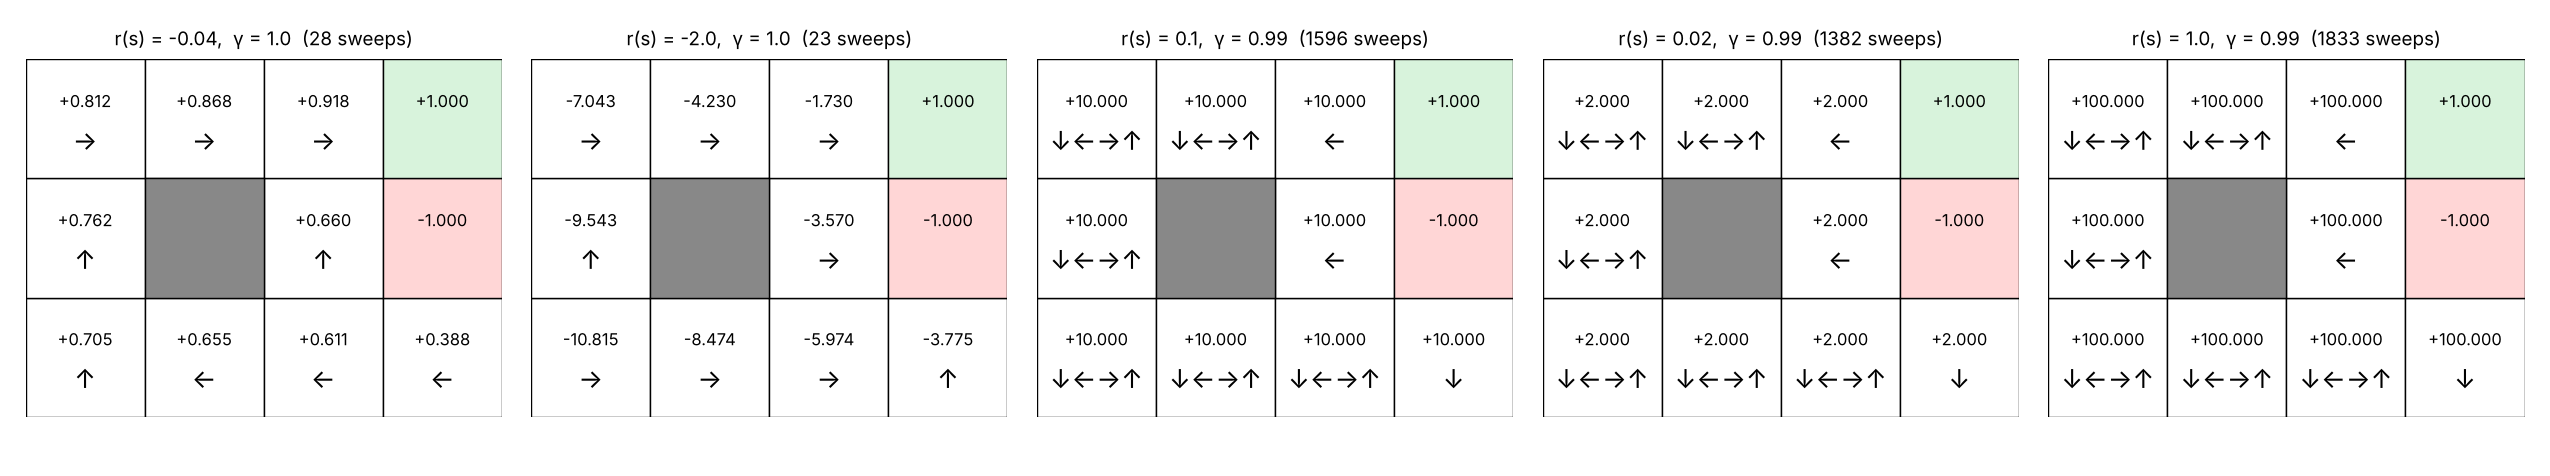
\includegraphics[width=\textwidth]{gridworld_policies.png}
\caption{Utilities and optimal policies of the $4\times3$ world for five living rewards (several
arrows mark ties).}
\label{fig:grid}
\end{figure*}

\subsection{Gbike: formulating the MDP}
The Gbike problem is Jack's car rental from Sutton and Barto \cite{sutton2018} in a bicycle setting.
We formulate it as a continuing finite MDP:
\begin{itemize}
\item \textbf{Time step}: one day; discount $\gamma=0.9$.
\item \textbf{State} $s=(n_1,n_2)$: bikes at each location at the end of the day, $0\le n_i\le20$,
so $|S|=441$.
\item \textbf{Action} $a\in\{-5,\dots,5\}$: the net number of bikes moved overnight from location 1
to location 2, feasible if $a\le n_1$, $-a\le n_2$ and no location ends above 20.
\item \textbf{Dynamics}: the morning stocks are $m_1=n_1-a$ and $m_2=n_2+a$. Requests
$Q_i\sim\mathrm{Poisson}(3), \mathrm{Poisson}(4)$ are served up to the stock, and returns
$B_i\sim\mathrm{Poisson}(3),\mathrm{Poisson}(2)$ become available the next day:
$n_i' = \min\bigl(m_i - \min(Q_i,m_i) + B_i,\; 20\bigr)$.
\item \textbf{Reward}: $r = 10\bigl(\min(Q_1,m_1)+\min(Q_2,m_2)\bigr) - 2|a|$.
\end{itemize}
Given the action, the two locations evolve independently, so the expected value of the next state
factorises into matrix products:
\begin{equation}
\mathbb{E}\bigl[V(s')\mid s,a\bigr] = \mathbf{P}_1[m_1,:]\;V\;\mathbf{P}_2[m_2,:]^{\top},
\end{equation}
where $\mathbf{P}_i[m,n']$ is the probability of ending the day with $n'$ bikes starting from $m$.
We compute $\mathbf{P}_i$ exactly, putting all the Poisson tail mass of demand into ``rent
everything'' and all the excess returns into ``full at 20''.

\emph{Comparison with the provided code.} The MATLAB code in \st{gbike.zip} uses the same states,
actions, rewards and transition structure (rentals first, then returns, capped at 20). It differs
in three implementation details: it truncates the Poisson sums at 12, 14, 12 and 9 without
renormalising, so a little probability mass is lost; it evaluates the policy with a tolerance of
$\theta=0.1$; and it accumulates the expected reward inside the innermost of four nested loops,
which is correct but slow. Our version computes exact tails, uses $\theta=10^{-4}$ and vectorises
the expectation, and runs both problems in about four seconds.

\subsection{Policy iteration}
Policy iteration \cite{howard1960,sutton2018} alternates two steps until the policy stops changing.
\emph{Policy evaluation} solves $V^\pi(s) = \sum_{s'}P(s'\mid s,\pi(s))\bigl[r + \gamma V^\pi(s')\bigr]$
by repeated in-place sweeps until the largest change is below $\theta$. \emph{Policy improvement}
then sets $\pi(s)\leftarrow\arg\max_a q^\pi(s,a)$. Because there are finitely many policies and each
improvement is strict until the optimum is reached, the method terminates with an optimal policy,
usually in very few iterations.

\emph{Original problem.} Starting from ``never move'', policy iteration converged after 5
evaluation--improvement cycles (Fig.~\ref{fig:gbike}). The optimal policy moves bikes from
location 1 to location 2 (in 128 states) when location 2, which has the higher demand, is short,
and the other way (in 43 states) only when location 1 is nearly empty and location 2 is well
stocked. The optimal value ranges from 421 at $(0,0)$ to 637 at $(20,20)$, with $V(10,10)=574.9$;
the shape of the value surface and of the final policy match the textbook figure for Jack's car
rental.

\emph{Modified problem.} With the free first shuttle from location 1 to 2 and the INR 4 charge for
keeping more than 10 bikes at a location, policy iteration converged in 4 cycles and the policy
changed in 242 of the 441 states. Two effects are visible. First, moving one bike from 1 to 2 now
costs nothing, so the policy moves at least one bike in that direction in far more states (250
instead of 128). Second, the parking charge creates a ridge at 10--11 bikes: whenever a location
would hold just over 10 bikes, the policy moves the excess to the other location, so the policy
regions now have sharp corners at 10. The value at $(10,10)$ rises to 581 because of the free
shuttle, while the value at $(20,20)$ falls from 637 to 603 because both locations pay for a second
lot.

\begin{figure*}[t]
\centering
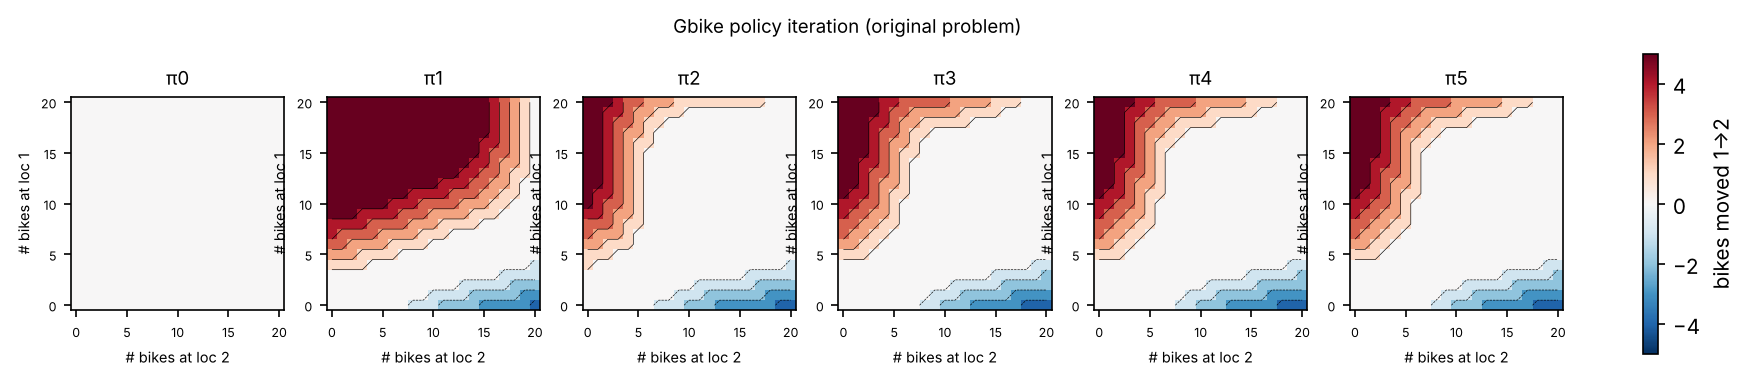
\includegraphics[width=0.49\textwidth]{gbike_policies_original.png}\hfill
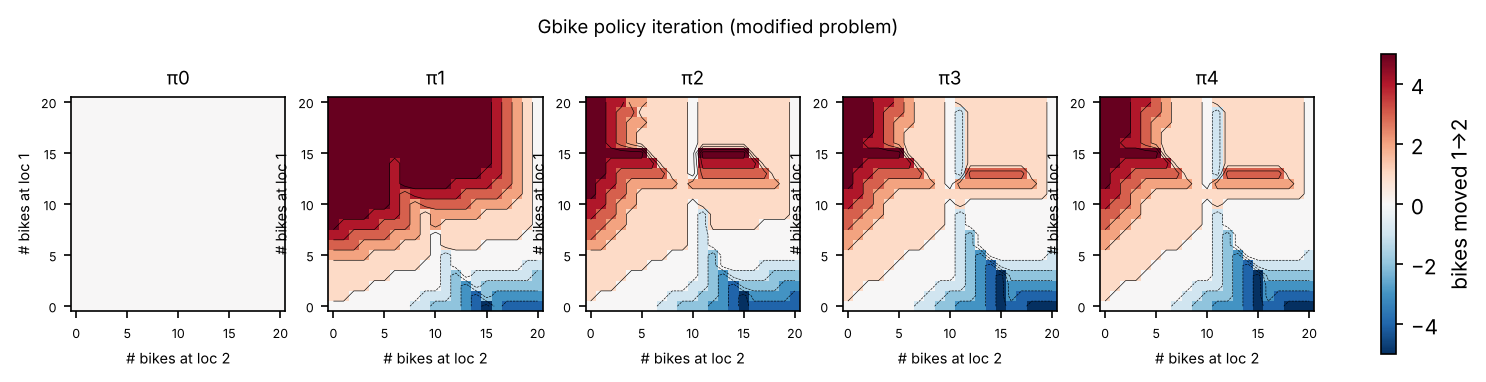
\includegraphics[width=0.49\textwidth]{gbike_policies_modified.png}\\[2pt]
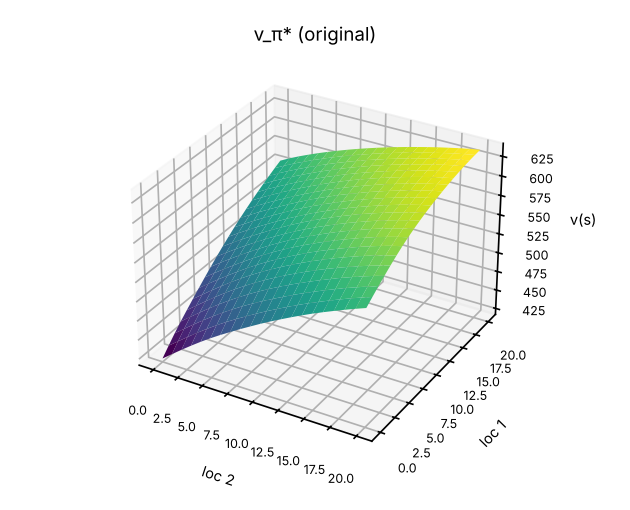
\includegraphics[width=0.3\textwidth]{gbike_value_original.png}\qquad
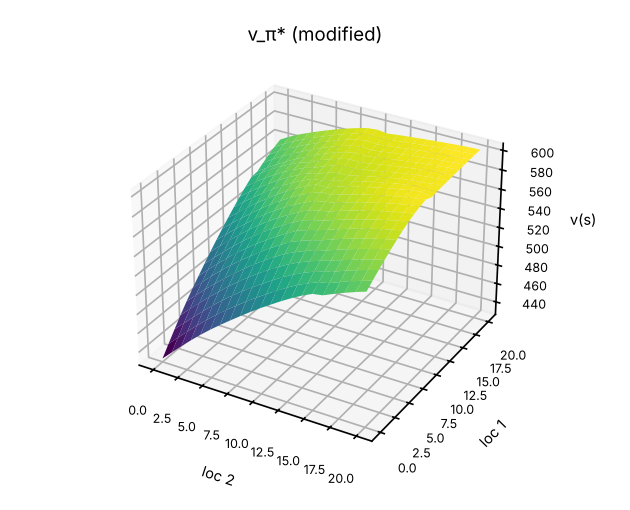
\includegraphics[width=0.3\textwidth]{gbike_value_modified.png}
\caption{Policy iteration for Gbike. Top: the sequence of policies for the original (left) and
modified (right) problems; red moves bikes from location 1 to 2, blue from 2 to 1. Bottom: the
optimal value functions.}
\label{fig:gbike}
\end{figure*}

%=====================================================================================
\section{Conclusion}
%=====================================================================================
The four labs share one idea: write down a probabilistic or energy-based model, and an algorithm
follows. The HMM's Markov assumption is what makes forward--backward and Viterbi efficient, and its
transition matrix turns regime inference into regime forecasting. A Hopfield network does whatever
its energy says, which is why it solves the eight-rook problem perfectly but the TSP only
unreliably. In bandits, the update rule embodies an assumption about the world: sample averages
assume stationarity, constant step sizes do not. And in MDPs, the Bellman equation turns
long-term planning into a sequence of one-step look-aheads, with the reward function setting the
agent's attitude to risk.

\bibliographystyle{IEEEtran}
\bibliography{refs}

\end{document}
